\scanpage{135}
\diagram{\begin{tikzcd}[ampersand replacement=\&,row sep=small,column sep=small]
X\arrow[dd]\&\&X'\arrow[ll]\arrow[dd]\&\\
\&X_{/y}\arrow[ul]\arrow[dd,"\text{coasph.}"]\&\&X'_{/y'}\arrow[ll]\arrow[ul]\arrow[dd,"\text{coasph. ?}"]\\
Y\&\&Y'\arrow[ll,"{\deleted{\text{\unsure{lisse}}}}"]\&\\
\&Y_{/y}\arrow[ul]\&\&Y'_{/y'}\arrow[ll,"{\substack{\deleted{\text{lisse à fibres}}\\\text{asph.}}}"]\arrow[ul]
\end{tikzcd}}

Catégories sur $\Delta^2$ (\unsure{motivé} par question du \unsure{composé|comportement} des $W^{\unsure{u|n}}$)

\diagram{\begin{tikzcd}[ampersand replacement=\&,row sep=small,column sep=small,execute at end picture={\draw ([xshift=-6pt,yshift=7pt]a.north west) to[out=0,in=85] ([xshift=5pt]b.east);}]
|[alias=a]|X_0\arrow[dr,dash,"{\substack{\text{coét}\\\text{asph.}\\\text{i.e iso}}}"'] \&\\ \&|[alias=b]|X_1
\end{tikzcd}}

\diagram{\begin{tikzcd}[ampersand replacement=\&]
X\&\\ {}\arrow[r,very thick]\&{}
\end{tikzcd}}

\diagram{\begin{tikzcd}[ampersand replacement=\&,row sep=small,column sep=small]
X\arrow[d,"\text{coasph.}"']\&X'\arrow[l]\arrow[d,"\text{coasph. ?}"]\&\\
Y\&Y'\arrow[l,"{\substack{\text{lisse}\\\text{à fibres}\\\text{asph.}}}"]\&\\
{}_{y\backslash}Y\arrow[u]\&\&{}_{y'\backslash}Y'\arrow[ul]\arrow[ll]
\end{tikzcd}}

\[
\begin{aligned}
 &\deleted{\unsure{\Delta^2}}\\
 &X_{01}\qquad X_{12}\qquad X_{02}
\end{aligned}
\]

\diagram{\begin{tikzcd}[ampersand replacement=\&,row sep=small,column sep=small]
\&X_1\arrow[dr]\&\\
\unsure{\alpha|X}_{01}\arrow[ur,dash]\arrow[dd,leftrightarrow,"\unsure{a}"]\&\&X_{12}\\
\&\deleted{\unsure{X}}\arrow[uu]\arrow[dl]\arrow[dr]\&\\
X_0\arrow[dr]\&\&X_2\arrow[uu]\arrow[dl]\\
\&X_{0,\unsure{2}}\&
\end{tikzcd}}

\figure{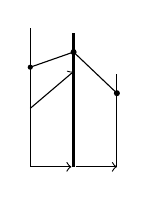
\begin{tikzpicture}[scale=.55]
\draw (0,0)--(0,3.2); \draw[very thick] (1,0)--(1,3.1); \draw (2,0)--(2,2.15);
\draw[->] (0,0)--(.95,0); \draw[->] (1.05,0)--(2,0);
\draw (0,2.3)--(1,2.65)--(2,1.7); \draw[->] (0,1.35)--(1,2.2);
\fill (0,2.3) circle (.06) (1,2.65) circle (.07) (2,1.7) circle (.07);
\end{tikzpicture}}

\diagram{\begin{tikzcd}[ampersand replacement=\&,row sep=small,column sep=small,cells={font=\scriptsize}]
\&\overset{\text{asph.}}{X_{02}}\arrow[dd,"W"]\&X_2\ \text{asph}\arrow[l,"{\deleted{\unsure{W}}}"]\arrow[dd,"W"]\\
\text{asph. }X_0\arrow[ur,"\text{asph}"]\arrow[dd,"\text{asph}"']\&\&\\
\&\underset{\text{asph.}}{X_{012}}\&X_{12}\ \text{asph}\arrow[l,"W"]\\
\text{asph }X_{01}\arrow[ur,"W"]\&\&\\
\&\underset{\text{asph.}}{X_1}\arrow[ul,"W"']\arrow[uur,"\text{asph.}"']\&
\end{tikzcd}}

\diagram{\begin{tikzcd}[ampersand replacement=\&,row sep=small,column sep=small,cells={font=\scriptsize},execute at end picture={\draw ([xshift=-4pt,yshift=2pt]z.north west) -- ++(0.65,1.8);}]
\&\&\&\&\widetilde X_{0\unsure{2|7}}\arrow[dddd,bend left=45]\\
\&\&\overset{\text{asph}}{\widetilde X'_{02}}\arrow[urr]\arrow[ddl,"\text{\unsure{Catfib}}"']\arrow[ddr,leftrightarrow,"{\text{\unsure{Catcof}}}","{\underline{\text{asph}}}"']\&\&\\
\&\&\&\&\\
\&\text{asph. }\widetilde X_{01}\arrow[dl,"\text{\unsure{Catfib}}"']\arrow[dr,"{\text{Cof}}","{\underline{\text{asph}}}"']\&\&\widetilde X_{12}\ \text{asph.}\arrow[dl,"\text{fib}"']\arrow[dr,"{\text{\unsure{Catcof}}}","{\underline{\text{asph}}}"']\&\\
|[alias=z]| \underset{\text{asph}}{X_0}\&\&\underset{\text{asph}}{X_1}\&\&\underset{\substack{\text{asph,}\\\text{(objet final)}}}{X_2}
\end{tikzcd}}
% archive sheet number: 135
